\section{Simulation Results}
The path following algorithm has been tested in the same path and considering different settings for the algorithm. In all cases, the distance in which the active waypoints are changed is \num{1} m. For seeing the results, the nonlinear model of the system has been simulated with the path following algorithm and the two inner controller designs. In the plots presented, the data from 100 simulations is depicted, where the disturbances, model uncertainties and noise affect the system.

The wind disturbance varies randomly from $\pm$\num{1.5} N in force along $x_\mathrm{b}$ and $y_\mathrm{b}$ and from $\pm$\num{1.5} Nm in torque in $\psi$. The waves are assumed to be sinusoidal with amplitude of 1N and a frequency that goes from 0 to 10 Hz. This disturbance is applied along $x_\mathrm{b}$ and $y_\mathrm{b}$. 

The uncertainty considered is of 20\% in all parameters of the model, that is, the added masses, $m_\mathrm{x}$ and $m_\mathrm{y}$, the moment of inertia around the $z_\mathrm{b}$ axis, $I_\mathrm{z}$, the damping coefficients, $d_\mathrm{x}$, $d_\mathrm{y}$ and $d_\psi$, and the vessel lengths, $l_1$ and $l_2$.  

In \autoref{fig:lqrwrong}, \ref{fig:distlqrwrong}, \ref{fig:robwrong} and \ref{fig:distrobwrong} the results of the algorithm are presented by depicting the path taken by the vessel and the distance to the target path. In these figures, the path following algorithm corresponds to the simpler case in which $\psi_\mathrm{ref} = \chi$, that is, assuming the velocity of the vessel is pointing along the $x_\mathrm{b}$ direction. The simulations are performed with both inner controller designs. 

\begin{figure}[H]
	\captionbox  %<--use captionbox instead if no global caption is needed
	{  
		Performance of the path following algorithm based on $\psi_\mathrm{ref}=\chi$ and using the LQR inner controller. The system is experiencing wind and wave disturbances, model perturbations and measurement noise.\label{fig:lqrwrong}                                
	}                                                                 
	{                                                                  
		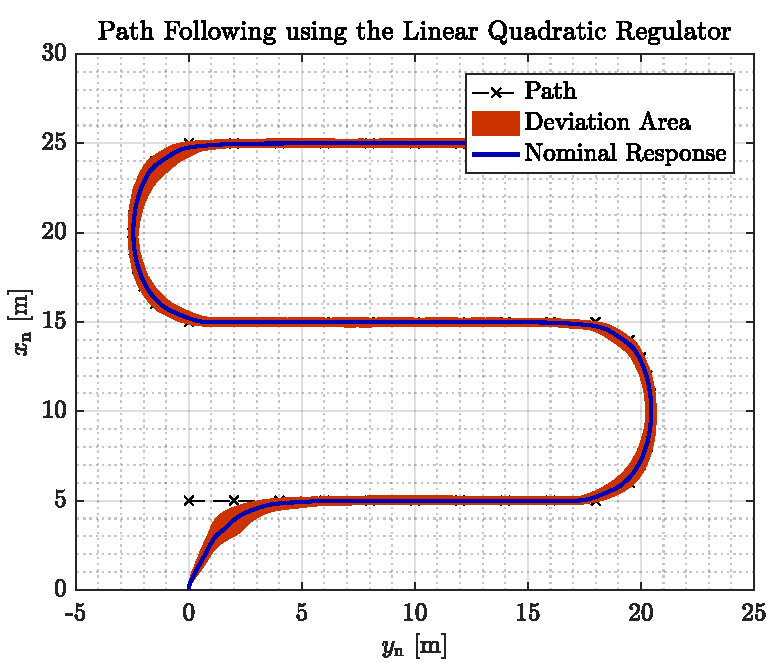
\includegraphics[width=.45\textwidth]{figures/path_lqr_no_correc}         
	}                                                                    
	\hspace{5pt}                                                  
	\captionbox
	{       
		Distance to the path when using the algorithm based on $\psi_\mathrm{ref}=\chi$ and the LQR inner controller .The system is experiencing wind and wave disturbances, model perturbations and measurement noise.
		\label{fig:distlqrwrong}                               
	}                                                                  
	{                                                                    
		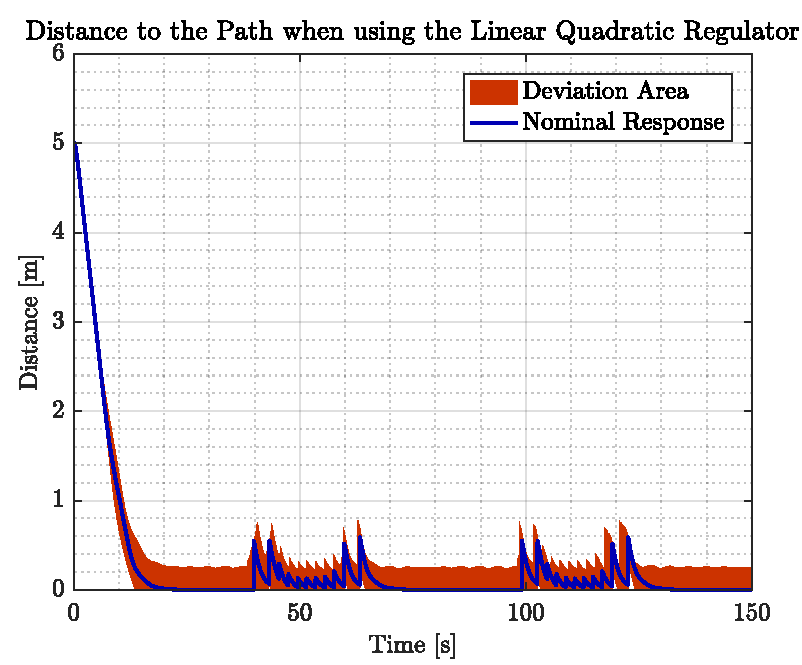
\includegraphics[width=.45\textwidth]{figures/dist_lqr_no_correc}         
	}                                                                         
\end{figure}
\begin{figure}[H]
	\captionbox 
	{   
		Performance of the path following algorithm based on $\psi_\mathrm{ref}=\chi$ and using the $\mathcal{H}_\infty$ inner controller. The system is experiencing wind and wave disturbances, model perturbations and measurement noise.\label{fig:robwrong}
	}                                                                 
	{                                                                  
		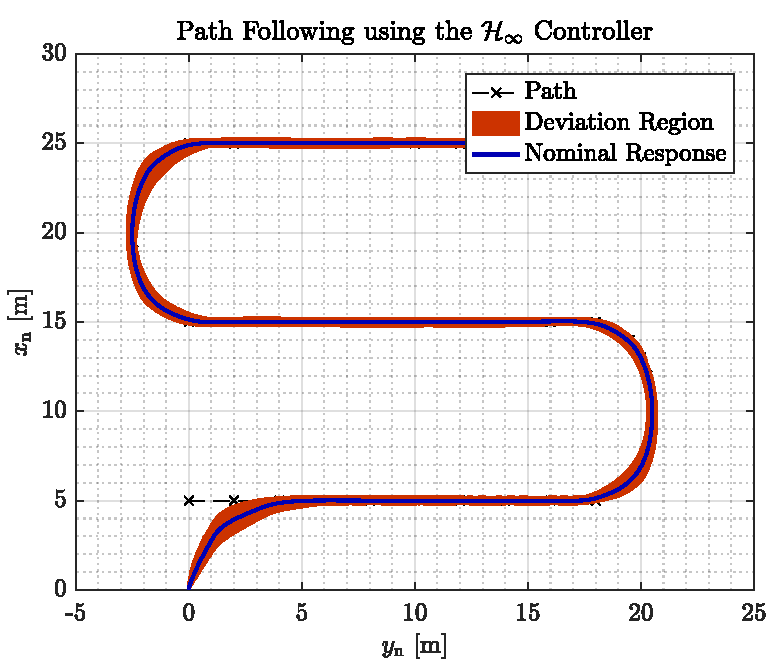
\includegraphics[width=.45\textwidth]{figures/path_rob_no_correc}         
	}                                                                    
	\hspace{5pt}                                                          
	\captionbox  
	{      
		Distance to the path when using the algorithm based on $\psi_\mathrm{ref}=\chi$ and the $\mathcal{H}_\infty$ inner controller .The system is experiencing wind and wave disturbances, model perturbations and measurement noise.\label{fig:distrobwrong}
	}                                                                          
	{
		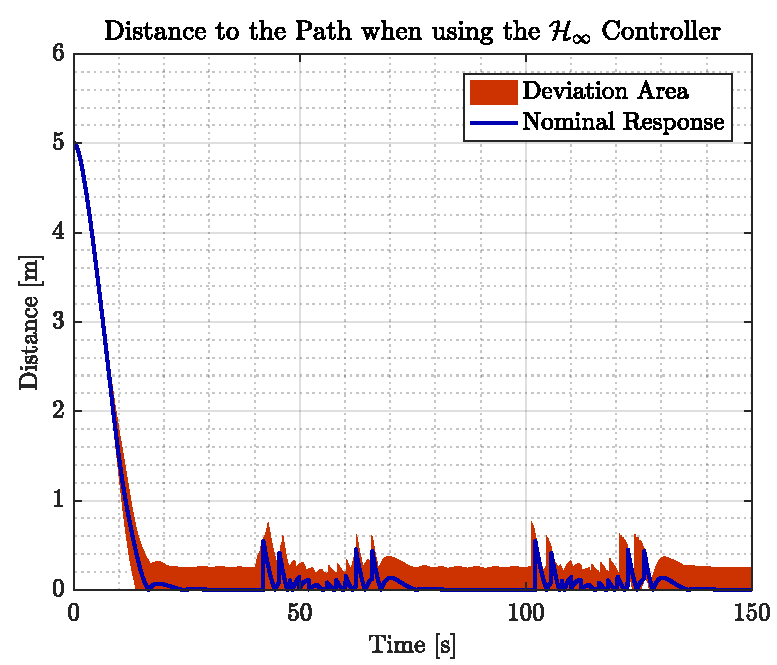
\includegraphics[width=.45\textwidth]{figures/dist_rob_no_correc}
	}
\end{figure}

In these graphs, it is clear that the path is not precisely followed when disturbances are introduced in the system. This offset is expected as the assumption for this simpler algorithm to work does not hold with disturbances like wind and waves. The latter is specially visible in the straight line parts of the path, where the vessel movement shows a 1-$\sigma$ value that goes up to 15 cm and a maximum value that reaches up to approximately 40 cm.

The straight path limits are also included to show the parts of the path where it is important to be closed to the line. It can be seen that both nominal responses and the 1-$\sigma$ regions are below 40 cm.

When the information of the vessel velocity is used to calculate the reference angle, $\psi_\mathrm{ref}$, the disturbance is rejected. This is seen in \autoref{fig:lrqcorrect}, \ref{fig:distlqr}, \ref{fig:robustcorrect} and \ref{fig:distrobustcorrect}, where the vessel is experiencing disturbances and model perturbations in the same range as in the previously shown figures. Both the vessel X-Y movement and the distance to the target path are depicted. 

\begin{figure}[H]
	\captionbox  %<--use captionbox instead if no global caption is needed
	{               %                                \%-%-%-%-%-%-%\
		Performance of the path following algorithm based on $\psi_\mathrm{ref}=\chi-\beta$ and using the LQR inner controller. The system is experiencing wind and wave disturbances, model perturbations and measurement noise.                %\
		\label{fig:lrqcorrect}                                  %\
	}                                                                 %\
	{                                                                  %\
		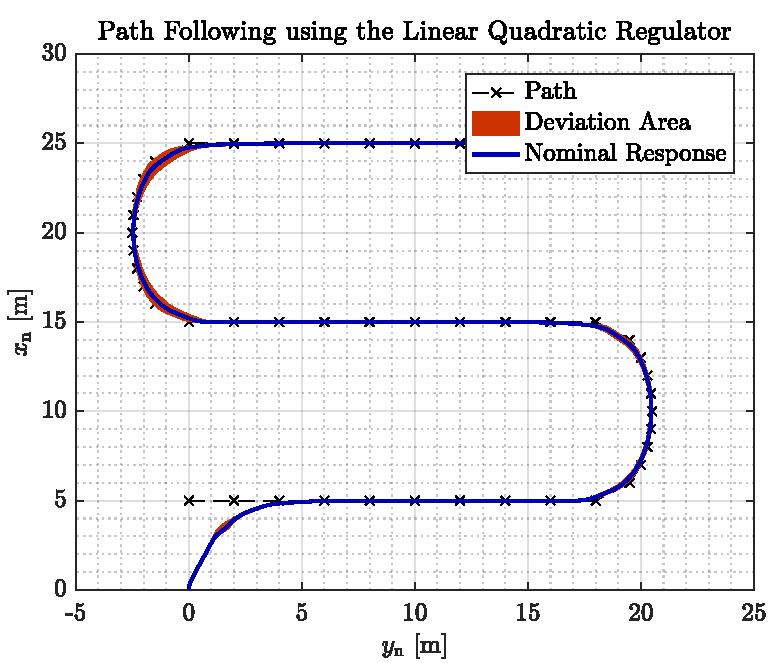
\includegraphics[width=.45\textwidth]{figures/path_lqr}         %\
	}                                                                    %\
	\hspace{5pt}                                                          %\
	\captionbox  %<-----------------------------------------------------%\
	{       
			Distance to the path when using the algorithm based on $\psi_\mathrm{ref}=\chi-\beta$ and the LQR inner controller .The system is experiencing wind and wave disturbances, model perturbations and measurement noise.                                                                  %\                         %\
		\label{fig:distlqr}                                     %\
	}                                                                           %\
	{                                                                            %\
		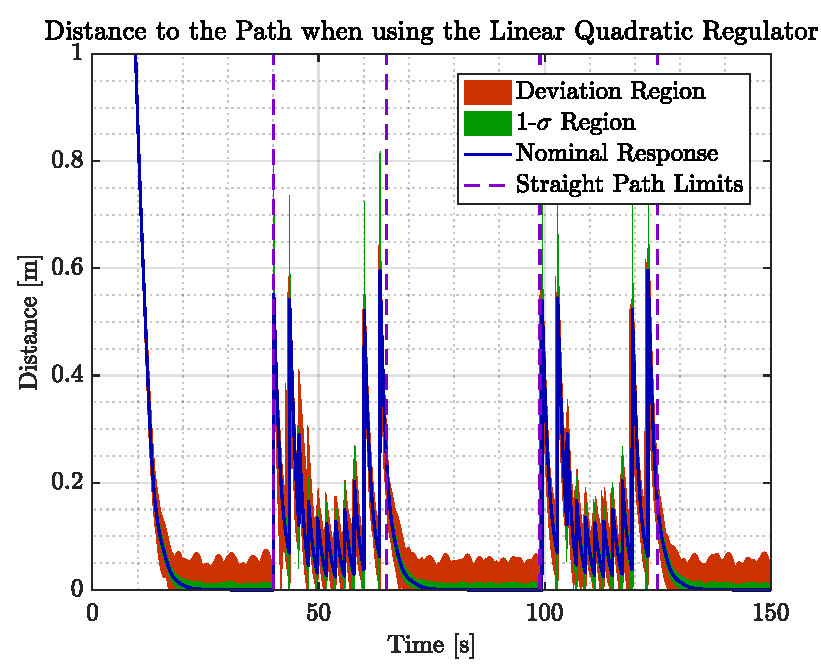
\includegraphics[width=.45\textwidth]{figures/dist_lqr}            %|
	}                                                                             %|
\end{figure}
\begin{figure}[H]
	\captionbox 
	{   
		Performance of the path following algorithm based on $\psi_\mathrm{ref}=\chi-\beta$ and using the $\mathcal{H}_\infty$ inner controller. The system is experiencing wind and wave disturbances, model perturbations and measurement noise. \label{fig:robustcorrect}
	}                                                                 
	{                                                                  
		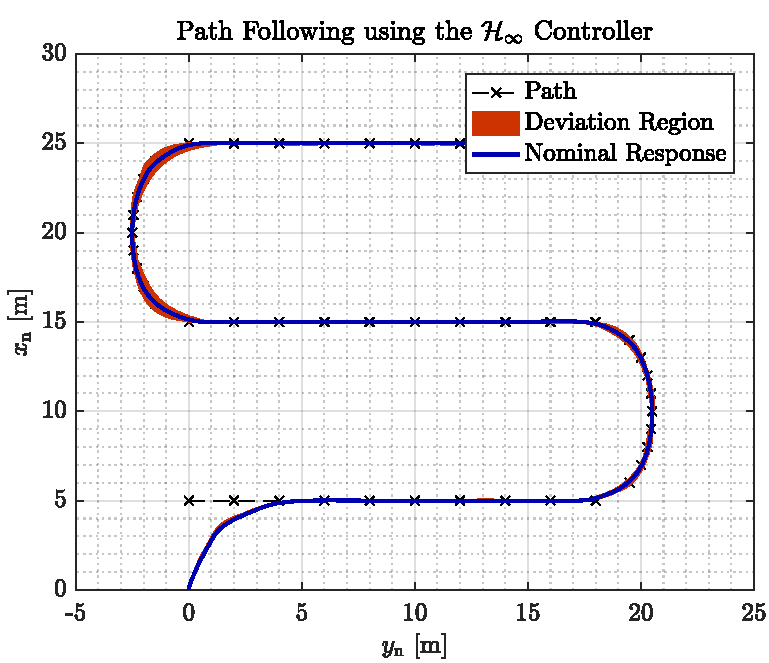
\includegraphics[width=.45\textwidth]{figures/path_rob}         
	}                                                                    
	\hspace{5pt}                                                          
	\captionbox  
	{      
			Distance to the path when using the algorithm based on $\psi_\mathrm{ref}=\chi-\beta$ and the $\mathcal{H}_\infty$ inner controller .The system is experiencing wind and wave disturbances, model perturbations and measurement noise.\label{fig:distrobustcorrect}
	}                                                                          
	{
		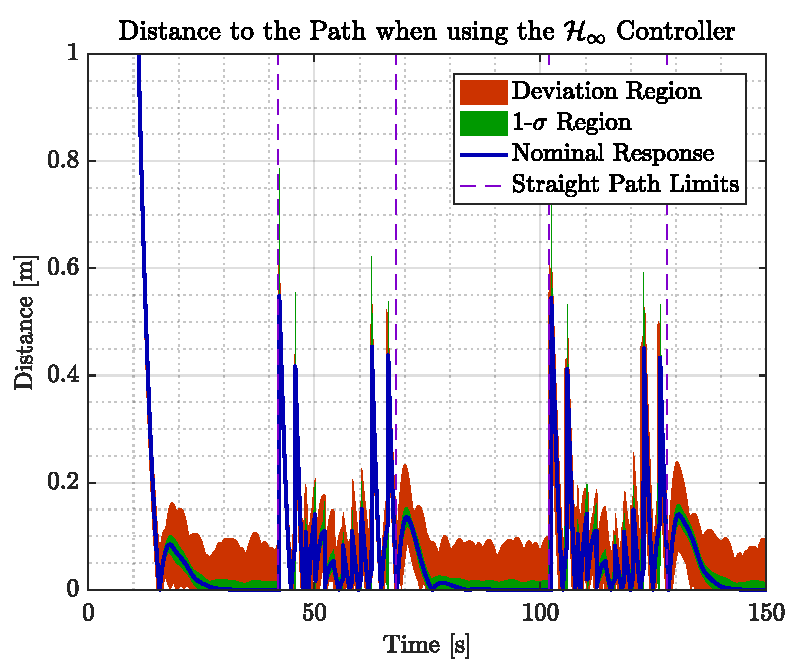
\includegraphics[width=.45\textwidth]{figures/dist_rob}
	}
\end{figure}

In this case, the offset in position has been corrected and the path is followed within the desired precision in the straight line segments. There are still some small deviations due to the wave disturbance present in the system, but the 1-$\sigma$ value is mostly 5 cm and the maximum variations stay below 15 cm with respect to the reference path.